\documentclass[conference]{IEEEtran}
\IEEEoverridecommandlockouts
% The preceding line only needs to identify funding in the first footnote. If that is unnecessary, please comment on it.
\usepackage{cite}
\usepackage{amsmath,amssymb,amsfonts}
\usepackage{algorithmic}
\usepackage{graphicx}
\usepackage{textcomp}
\usepackage{xcolor}
\usepackage{bm}
\def\BibTeX{{\rm B\kern-.05em{\sc i\kern-.025em b}\kern-.08em
    T\kern-.1667em\lower.7ex\hbox{E}\kern-.125emX}}
\begin{document}

\title{Autonomous Design Report FS-AI\\[-0.3em]
{\Large Atlas Racing - Heriot Watt University Dubai}\\[-0.6em]
}

\author{\IEEEauthorblockN{Joseph Abdo, Moaiz Saeed, Aditya Shibu, Abdul Maajid Aga and Apsara Sivaprazad}
}

\maketitle

\begin{abstract}
Autonomous racing presents unique perception challenges that demand high-precision environmental sensing with minimal latency. This Autonomous Design report documents our technical approach to developing a fully autonomous vehicle for the FS-AI UK competition. A key challenge we face is the unavailability of the ADS-DV vehicle in our home country, the UAE, which significantly limits our ability to test on the given hardware. As a result, all our systems are designed to be robust, modular, and adaptable, allowing for rapid iteration. For instance, we have implemented fallback pipelines to ensure we can at least showcase a functioning autonomous system under unforeseen conditions.
\end{abstract}

\section{Introduction}
Every year, Formula Student pushes the bounds of technology with its subsection Formula Student AI, which moves the bounds of autonomous race development, challenging universities to create high-speed racing environments without human intervention. These achievements are critical platforms for developing new talent and innovating autonomous technologies.
Atlas Racing from Heriot-Watt University Dubai sets out to face this unique challenge in developing an autonomous system for the FS-AI UK competition. The primary method for development is utilising a simulation-first development approach due to the limited access 
\section{System Architecture}
This section outlines the hardware and software architecture of the autonomous driving system deployed on the ADS-DV platform.  The entire software stack is developed using the Robot Operating System 2 (ROS 2) framework and runs on Ubuntu 22.04.

\subsubsection{Sensors Onboard}
The perception stack includes a ZED 2i stereo depth camera and a RoboSense Helios 3D LiDAR sensor. The stereo camera provides synchronized RGB and depth images, while the LiDAR sensor generates 3D point clouds, this allows for accurate spatial perception of the environment. For localization, the system is also equipped with an Inertial Measurement Unit (IMU) and a GPS module. 

\subsubsection{Computing Module}
All sensor data is processed on an NVIDIA Jetson Orin AGX module, which is the primary onboard computational unit. It is selected for its high-performance GPU capabilities and low power consumption, making it suitable for real-time data fusion. 

\subsubsection{Sensor Fusion}
Low-level fusion is performed on the inputs from the camera and LiDAR for cone detection. These detected features are essential for estimating the drivable space and forming a reliable map of the environment.  

\subsubsection{SLAM (Simultaneous localization and mapping)}
The system uses an Extended Kalman Filter (EKF) to estimate odometry by fusing data from the IMU, GPS, and LiDAR sensors. The odometry and the cone detections are provided to the Cartographer SLAM framework to perform real-time simultaneous localization and mapping. The output of Cartographer is a continuously updated global map that reflects the vehicle’s environment and position within it. 

The generated map is fed to the path planning module, which computes a sequence of waypoints to the current navigation objectives. This module sets environmental constraints and vehicle dynamics to ensure the generated trajectory is failsafe. 

\subsubsection{Navigation Control}
The final stage of the pipeline involves the navigation control module, which uses the computed waypoints to derive vehicle kinematics. It then generates wheel commands to steer, throttle, or brake the vehicle appropriately. These commands are transmitted to the ADS-DV platform via a Controller Area Network (CAN) bus interface, completing the control loop.

\section{Perception}
This section details the implementation of the vehicle's perception system, explaining how it interprets its environment using both Lidar (laser-based) and vision-based technologies.

\subsection{LiDAR (laser-based)}\label{AA}
We have selected the RoboSense Helios series Lidar with a 16-beam configuration, offering a balanced trade-off between angular resolution, detection range, update rate, and cost-effectiveness. We applied filtering and clustering techniques to enhance data reliability to remove irrelevant or noisy points that could interfere with path planning. Our code detection pipeline using Lidar follows a multistage approach, as outlined below:
\subsubsection{Raw Data Acquisition}
Data is captured as points in 3D space and transformed to the vehicle's reference frame using sensor\_transform matrices. We've then implemented a thread-based processing with Mut-Ex (Mutually Exclusive) locks to ensure thread safety while maintaining real-time performance.
\subsubsection{Point Cloud Filtering and Accumulation}
We employ several filtering strategies:
\begin{itemize}
    \item Distance-based filtering:
    \[
    \mathit{close\_points\_mask} = \left( d < 50.0 \right)
    \]
    Where \textbf{‘d’} is the distance to each point, this step filters out all points beyond 50 meters, allowing the system to focus on relevant track sections.

    \item Height-based filtering:
    \[
    \mathit{near\_ground\_mask} = \left( z < h_{\text{ground}} + 0.5 \right) \land \left( z > h_{\text{ground}} \right)
    \]
    where \textbf{‘z’} is the z-coordinate of the LiDAR points, and \textbf{‘$\bm{h_{\text{ground}}}$’} denotes the estimated ground height.

    \item Point accumulation: Points from multiple frames are appended to improve cone detection density, especially in sparse or occluded regions.
\end{itemize}

\subsubsection{Cone Identification}

Our approach uses DBSCAN clustering with the parameters eps=0.5 and min\_samples=5; we found this to be the sweet spot, which gave a good balance between noise reduction and the ability to detect distinct clusters in our data points. We selected DBSCAN over alternatives such as OPTICS because DBSCAN offers better computational efficiency at O(n log n) vs. O(n\textsuperscript{2}) \cite{b2}, which is critical for real-time performance. Although OPTICS provides more flexibility, since such granularity was unnecessary in our context, where cones are relatively uniform in size and spacing, DBSCAN effectively filters out noise while reliably clustering actual cone detections \cite{b1}.
\vspace{0.2em}
\subsubsection{Cone Validation}
We validate detected cones through size validation, ensuring that each cluster matches the expected physical dimensions of a cone. This is followed by confidence scoring, which evaluates point density and other cluster characteristics. Additionally, we have implemented multi-frame tracking to reduce false positives and enhance detection stability over time.

\vspace{0.4em}
This Lidar processing system maintains deterministic processing times below 100ms through efficient filtering and optimised algorithms such as DBSCAN. We've implemented 3d visualisation capabilities using Open3d and ROS visualisation markers for real-time debugging and development.

\subsection{Image and Object Detection (vision-based)}
Our object detection system is designed to accurately identify and classify the track cones in real-time while providing precise spatial information for navigation. After going through several approaches, we selected YOLOv8 as our primary detection model.

\subsubsection{Model Development and Training}
We used three cone datasets from Kaggle to create a unified training dataset with standardised labelling conventions. Our classification scheme used numeric labels (0=orange, 1=yellow, 2=blue, 3=large orange, and 4=unknown) to ensure consistent identification across various racing environments. The training process involved a train-test split of 80\% (10,003 images) 20\% (10\% validation, and 10\% testing, 1,250 images each) along with a training configuration with 100 epochs, 32 batches, and 25 early stopping patience. 

\begin{figure}[htbp]
\centerline{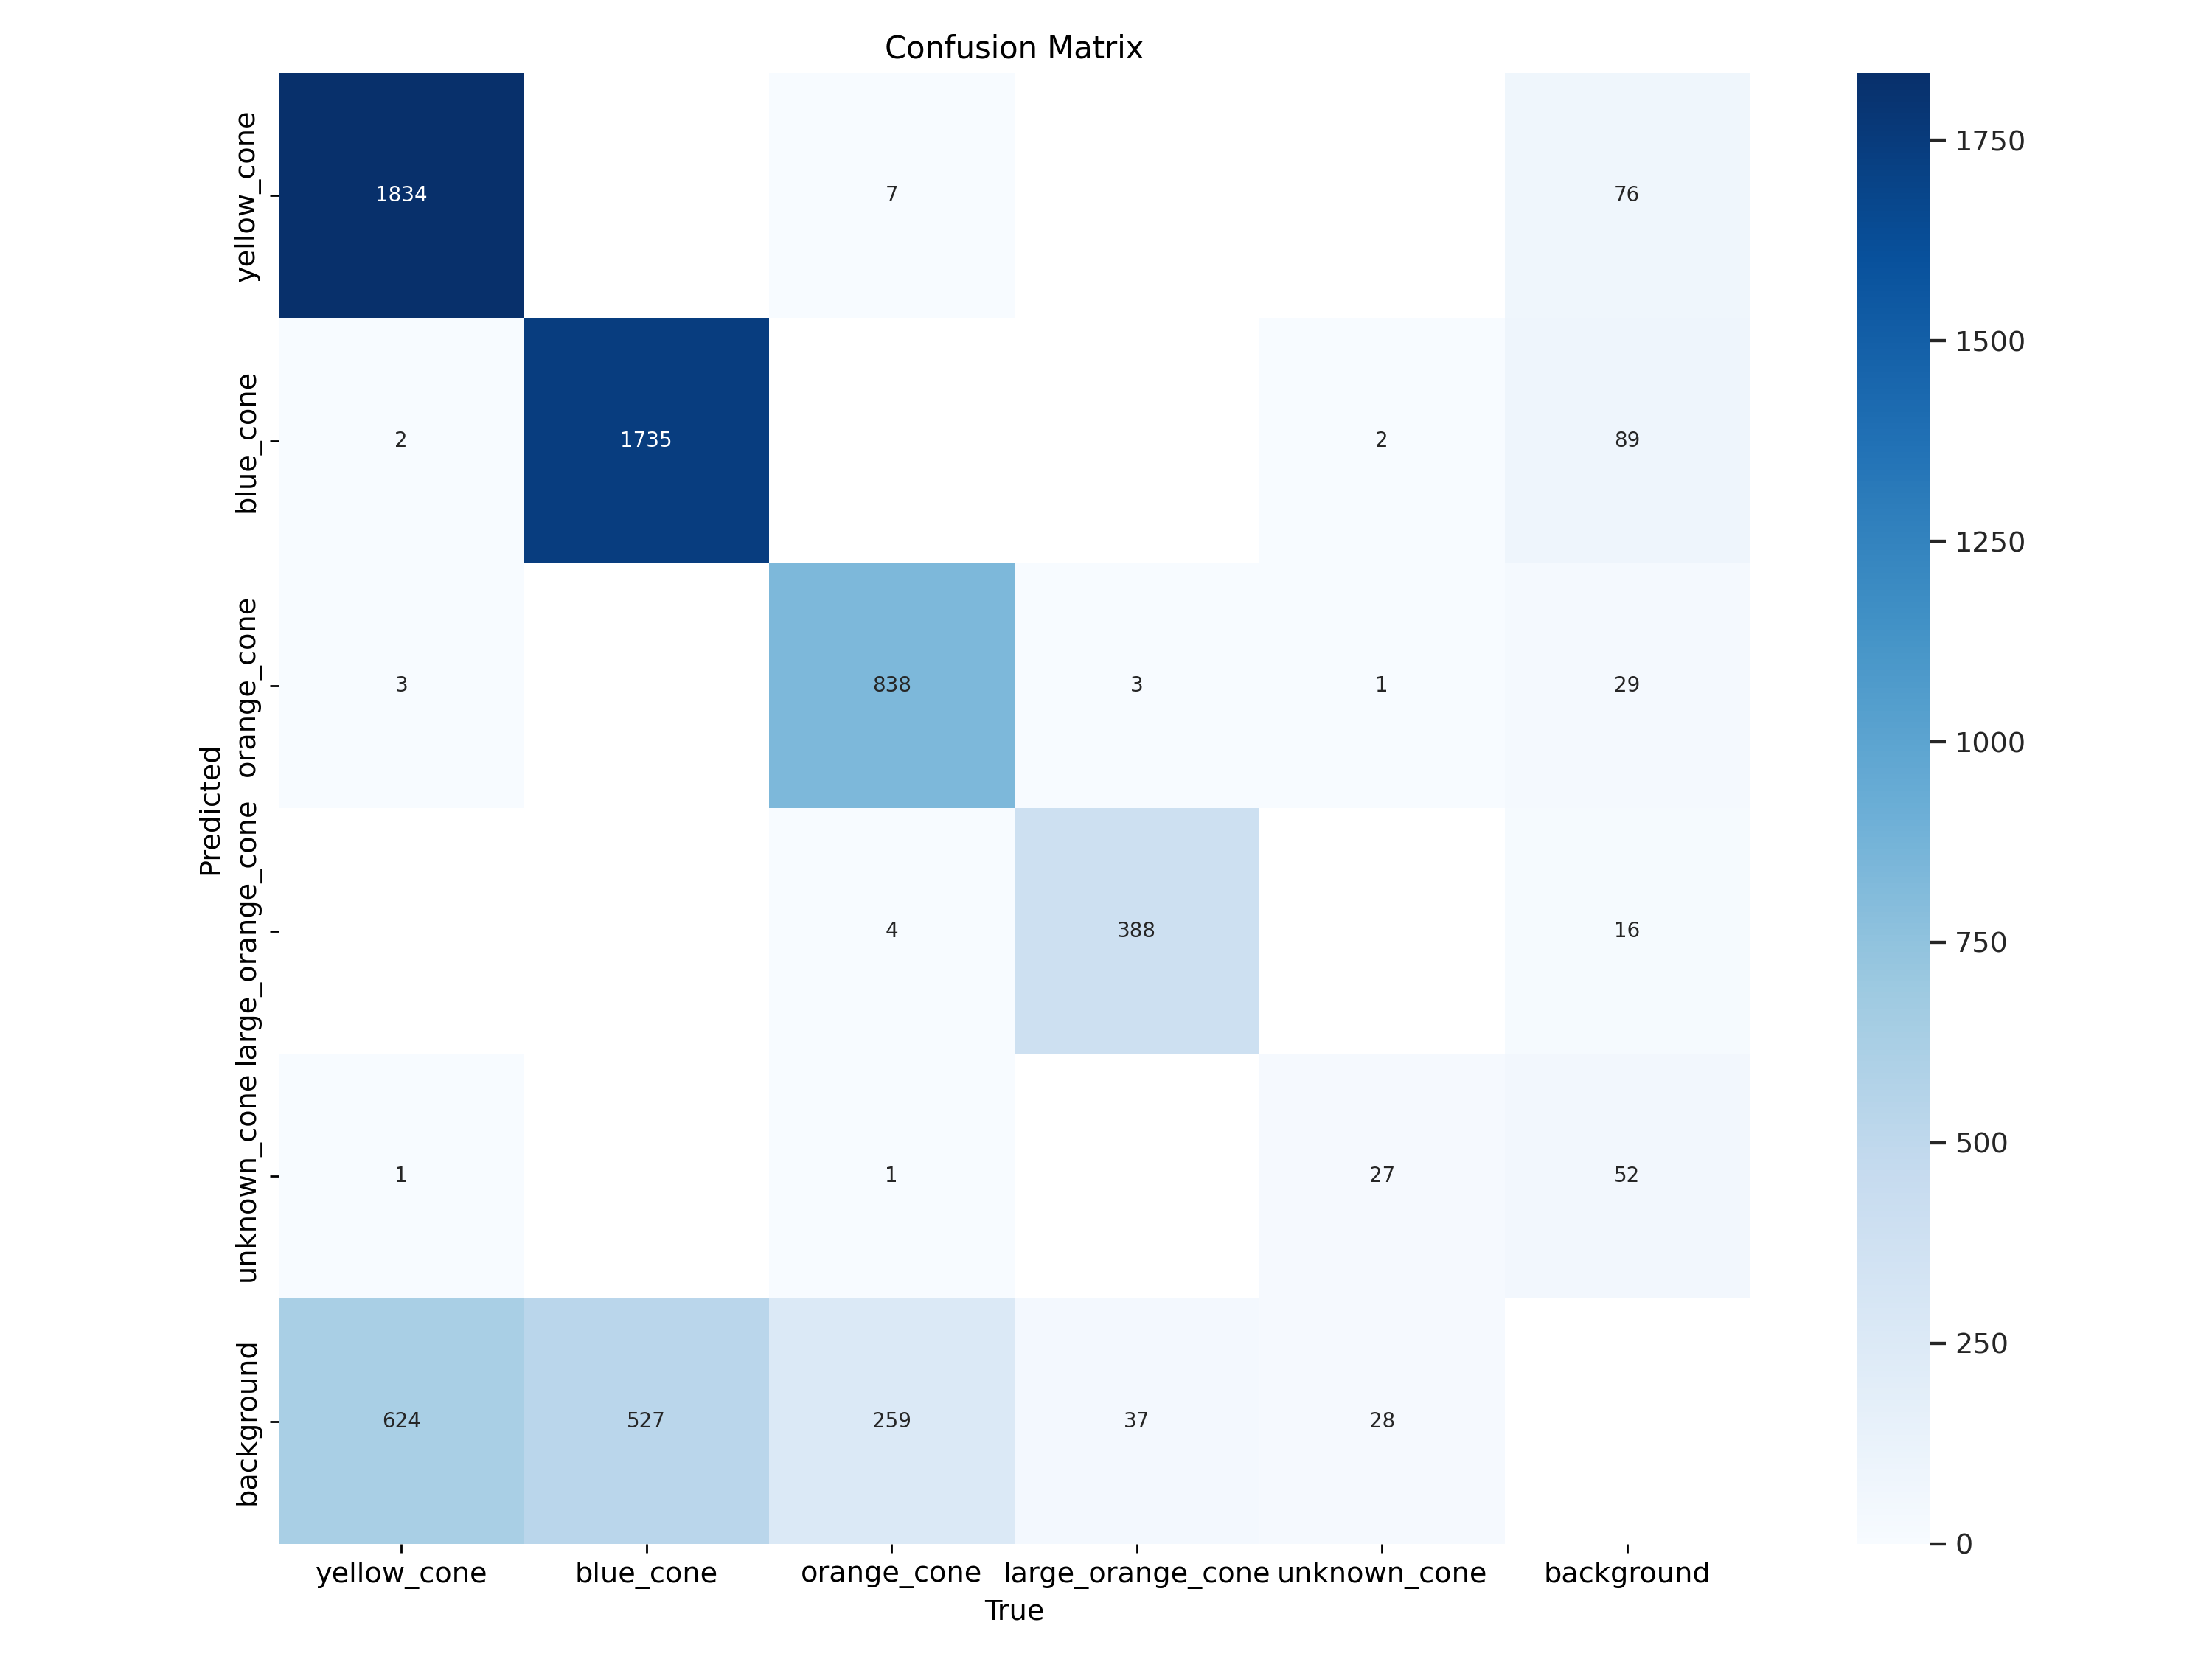
\includegraphics[scale=0.3]{confusion_matrix.png}}
\caption{Confusion Matrix of our trained YOLO Model}
\label{fig}
\end{figure}

\textbf{Testing Result:} The model accuracy is show in Figure 1, with appropriate results for yellow and blue cones (highest actual positive rates). The confusion matrices revealed that most misclassification occurred between visually similar cone types.

\subsubsection{YOLOv8 vs. HOG Performance Analysis}
We compared YOLO and Histogram of Oriented Gradients (HOG) with Support Vector Machines (SVMs), referencing Kaplan and Şaykol's research. While HOG with SVM achieved an 86.7\% success rate when trained on 80\% of the dataset, YOLO demonstrated superior reliability and accuracy in racing environments with significantly fewer false positives (5 vs. 84 for HOG), Higher actual positive detection rate (218 vs. 154 for SVM) and a better overall performance in dynamic racing environments.

\subsubsection{Performance metrics and Evaluation}
Our model evaluation demonstrated the relationship between confidence thresholds and detection accuracy. Our F1 score peaked between confidence thresholds of 0.1 and 0.6. Precision remained high across most confidence levels for all cone classes. Our recall started high at low confidence thresholds, stabilised between 0.6 and 0.4, and then dropped at higher thresholds.

\begin{figure}[htbp]
\centerline{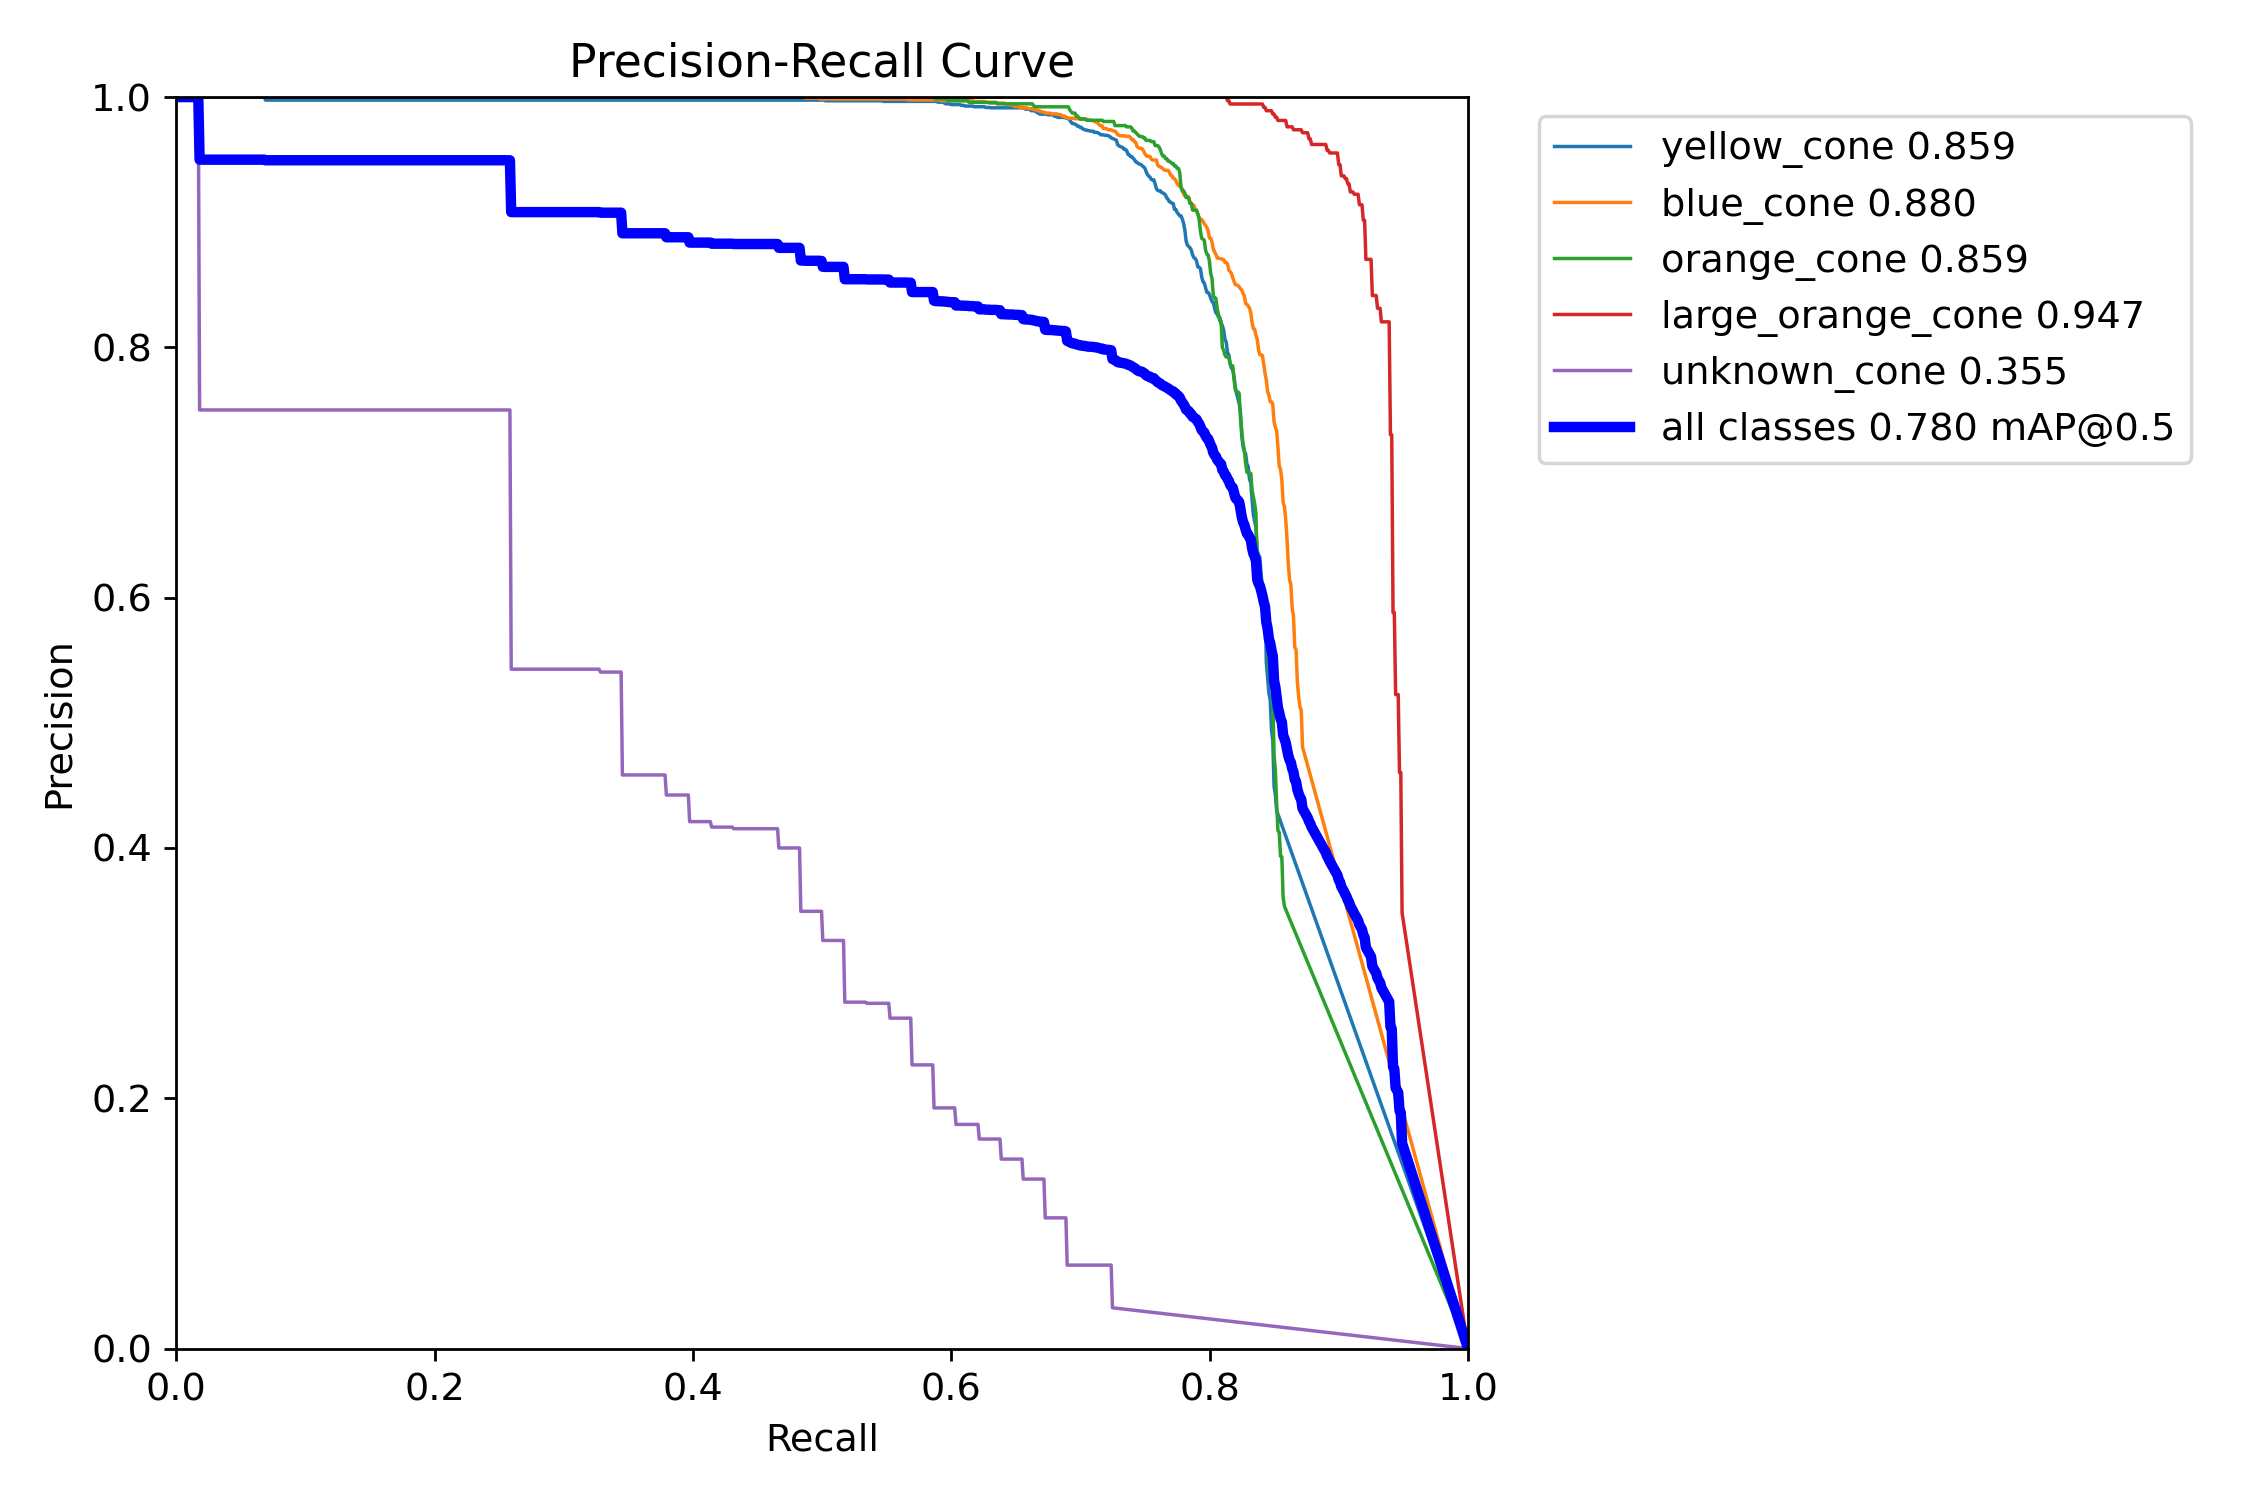
\includegraphics[scale=0.4]{PR_curve.png}}
\caption{Precision-recall curve}
\label{fig}
\end{figure}

\begin{figure}[htbp]
\centerline{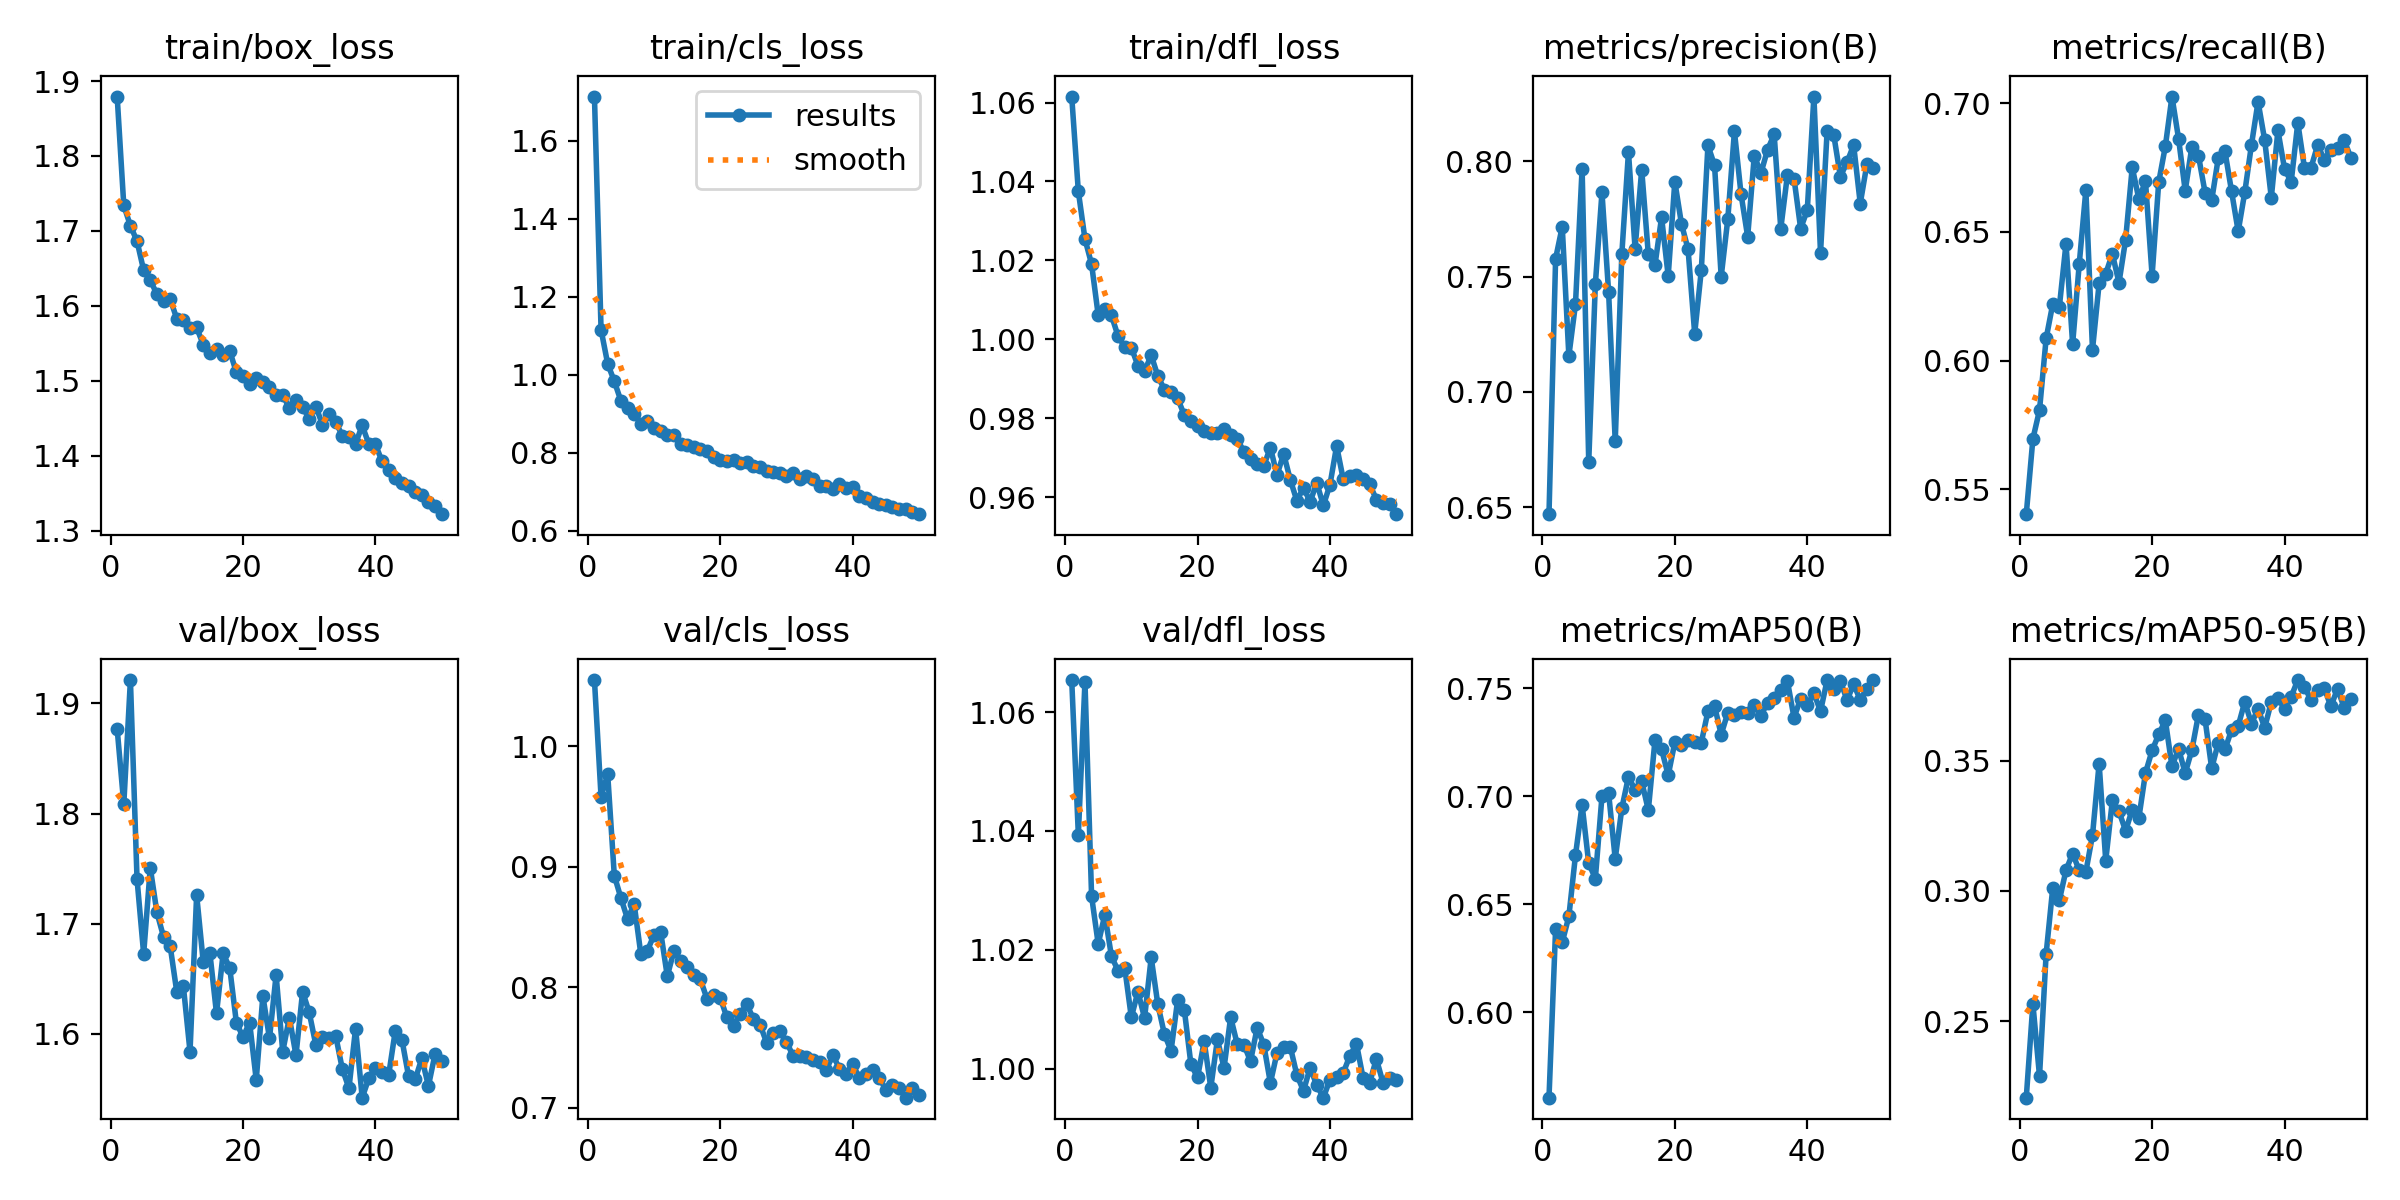
\includegraphics[scale=0.3]{results.png}}
\caption{Training metrics graph}
\label{fig}
\end{figure}

The precision-recall curve (Figure 2) illustrates the trade-off between detection accuracy and coverage. Our training metrics (Figure 3) showed consistent improvement across epochs for bounding box loss, classification loss, and mean average precision (mAP), confirming stable training without significant overfitting.

\subsection{Depth Camera (vision-based)}
Our system utilises the ZED 2i stereo camera as a secondary perception pipeline to enhance system reliability through sensor fusion and to provide critical colour classification capabilities that complement our Lidar system. We selected the ZED 2i specifically for its built-in stereo capabilities that provide accurate depth measurements up to 20m, which is critical for our cone detection requirements. The camera subsystem consists of two primary components.

\subsubsection{Advanced Depth Estimation}
A key innovation in our system is a multi-faceted depth estimation approach that combines several techniques: direct depth sampling from the stereo camera's depth map, temporal smoothing using a sliding window of recent detections, position-based depth estimation, and box-size–normalized depth correction. The final depth is computed as:
\[
\textit{final\_depth} = 0.5 \cdot \textit{smoothed\_depth} + 0.5 \cdot \textit{position\_depth}
\]
This provides more reliable depth estimates than any single method alone. This approach is particularly effective at handling the rapidly changing distances encountered in racing scenarios.

\subsubsection{Track Boundary Visualization}
Our system automatically identifies and visualizes track boundaries by first classifying detected cones based on color (yellow, blue, and orange). The cones are then sorted by depth to determine their sequential order along the track. To form a visual representation of the track edges, lines are drawn between consecutive cones of the same color. This process provides clear visual feedback that supports both real-time path planning and offline validation, helping to ensure accurate and reliable vehicle navigation.

\vspace{0.4em}
Through extensive testing, we found this camera-based perception system achieves detection ranges of 1-20m with centimeter-level accuracy after calibration. The integration with our LiDAR system through sensor fusion not only improves overall detection reliability but also color-based cone detection that simplifies our path planning algorithm.

\subsection{Laser-vision Fusion}\vspace{-0.4em}
Our system employs a fusion technique to combine LiDAR data with camera detections, leveraging the strengths of both perception systems to create a more robust and reliable cone detection system.

\subsubsection{Low-level Fusion Approach}
While many autonomous racing solutions employ mid-level fusion due to its lower computational complexity, out system implements low-level fusion to achieve peak performance and racing speeds on track. This approach processes raw data from both sensors jointly before making detection decisions, providing key advantages such as enhanced detection accuracy through complementary sensor information, Improved reliability across a wide range of weather conditions, More precise spatial localization by combining depth information from multiple sources, and reduced false positives through cross-validation between sensors.

Although the low-level fusion approach is more computationally more demanding, it yields superior detection quality which is critical for the high-speed racing environment where precise cone positioning is essential for optimal path planning.

\subsubsection{Sensor Alignment and Calibration}
Our fusion pipeline begins with precise sensor alignment using Rigid transformation matrices between LiDAR and camera reference frames, Depth correction factors to address systematic biases in sensors measurements and Point cloud projection into the camera's image plane for visual correlation.

These calibration steps ensure that data from both sensors is accurately registered in a common coordinate frame before fusion occurs.

\subsubsection{Data Association and Fusion Algorithm}
The core of our fusion system is a matching algorithm that associates LiDAR-detected cone clusters with camera-detected bounding boxes using the following steps:
\begin{itemize}
\item Projection Step: Lidar points are transformed to the camera frame and projected onto the image plane using the camera's intrinsic parameters
\item Association: Each 3D point is matched with its corresponding 2D detection using a weighted distance metric that considers both spatial proximity and confidence scores
\item Confidence Fusion: For matched detections, a confidence-weighted averaging is performed using the equation:
\begin{equation}
P_{\text{fused}} = \frac{P_{\text{camera}} \cdot w_{\text{camera}} + P_{\text{LiDAR}} \cdot w_{\text{LiDAR}}}{w_{\text{camera}} + w_{\text{LiDAR}}}
\end{equation}
Where \textbf{‘P'} stands for the position and \textbf{‘w'} stands for the weight/confidence.
\item Classification Transfer: Color information from the camera detections is transferred to the corresponding LiDAR points
\item Unmatched Point Handling: Points detected by only one sensor are preserved but assigned a reduced confidence score to maintain the continuity of detection
\end{itemize}

\subsubsection{Adaptive Confidence Weighting}
Our system employs dynamic confidence weighting that adjusts based on sensor reliability under different conditions such as when Camera detection confidence is weighted higher in good lighting conditions, LiDAR measurements are prioritized in low-light environments or at longer distances. Distance-dependent weighting gives preference to camera for color classification and LiDAR for precise positioning, and Historical detection consistenncy is factored into confidence calculations.

This adaptive approach ensures optimal fusion performance across the diverse conditions that might be encountered during the competition.

\subsubsection{Performance Improvements}
Although we initially employed a mid-level fusion approach, we transitioned to a low-level fusion due to lower vehicle speeds. Specifically, the mid-level fusion method introduced delays as it required each sensor to independently detect and process data before fusion. By contrast, low-level fusion integrates raw sensor data prior to processing, significantly reducing latency. This shift resulted in several key improvements, including an extended detection range exceeding 20m, cone color classification accuracy above 98\%, reduced overall detection latency, and enhanced tracking continuity during temporary sensor occlusions.

These improvements directly translate to higher racing speeds and more accurate path planning, giving our vehicle a competitive edge.

\section{State Estimation}
State Estimation is used to generate an accurate mapping for the environment containing the cone positions detected during the first run. Which could then be used to create an optimized path around the track for the next run.

\section{Path Planning}
For our path planning, we decided to use the pure pursuit tracking algorithm to compute steering commands required for the vehicle to follow the desired path in real time. The method works by continuously selecting a goal point on the planned path ahead of the vehicle's current position at some lookahead distance \textbf{L\textsubscript{d}}. In our implementation, the algorithm features a lookahead distance of 2.5-5m that is adaptively adjusted based on the car's current velocity to improve tracking stability based on the path's curvature. The lookahead distance is calculated by:
\begin{equation}
L_d = K_{ld} \times V + L_{fc}
\end{equation}

Where \textbf{L\textsubscript{d}} is the dynamic lookahead distance, \textbf{L\textsubscript{ld}} is the speed gain constant, \textbf{V} is the instantaneous forward velocity of the vehicle and \textbf{L\textsubscript{fc}} is the minimum lookahead distance. 

Once the goal point is identified, the algorithm determines the required steering angle by using the formula:
\begin{equation}
\delta = \arctan\left(\frac{2L \sin(\alpha)}{L_d}\right)
\end{equation}

Where \textbf{L} is the wheelbase of the vehicle, $\alpha$ is the angular deviation between the vehicle's heading and the vector connecting the real axle to the lookahead point with \textbf{L\textsubscript{d}} being the lookahead distance.

The calculation is repeated for each control cycle, ensuring that the vehicle constantly aligns itself with the updated path based on the latest cone detections. Unlike map-based navigation systems, this implementation operates in a dynamic and unstructured environment where the vehicle is reliant solely on visual cone detection to build a local representation of the track. Hence, Pure Pursuit is preferred for its computational simplicity, low latency, and its closed-loop geometric control, that makes it robust to perception noise and irregular cone spacing. Once we have a run through the track once, and mapped out our environment, we can then move ahead and build an optimized path using algorithms such as MPC (Model Predictive Control).

\section{Navigation and Control}

\begin{table}[htbp]
\caption{Table Type Styles}
\begin{center}
\begin{tabular}{|c|c|c|c|}
\hline
\textbf{Table}&\multicolumn{3}{|c|}{\textbf{Table Column Head}} \\
\cline{2-4} 
\textbf{Head} & \textbf{\textit{Table column subhead}}& \textbf{\textit{Subhead}}& \textbf{\textit{Subhead}} \\
\hline
copy& More table copy$^{\mathrm{a}}$& &  \\
\hline
\multicolumn{4}{l}{$^{\mathrm{a}}$Sample of a Table footnote.}
\end{tabular}
\label{tab1}
\end{center}
\end{table}

\section*{Acknowledgment}

The preferred spelling of the word ``acknowledgment'' in America is without 
an ``e'' after the ``g''. Avoid the stilted expression ``one of us (R. B. 
G.) thanks $\ldots$''. Instead, try ``R. B. G. thanks$\ldots$''. Put sponsor 
acknowledgments in the unnumbered footnote on the first page.

\begin{thebibliography}{00}
\bibitem{b1}
Martin Ester, Hans-Peter Kriegel, Jörg Sander, and Xiaowei Xu, 
\emph{A Density-Based Algorithm for Discovering Clusters in Large Spatial Databases with Noise}, 
Proceedings of the 2nd International Conference on Knowledge Discovery and Data Mining (KDD), 1996, pp. 226–231.
\bibitem{b2}
Erich Schubert, Jörg Sander, Martin Ester, Hans-Peter Kriegel, and Xiaowei Xu, 
\emph{DBSCAN Revisited, Revisited: Why and How You Should (Still) Use DBSCAN}, 
Lecture Notes, Data Mining Course, Northeastern University, 2017. 
\bibitem{b3} I. S. Jacobs and C. P. Bean, ``Fine particles, thin films and exchange anisotropy,'' in Magnetism, vol. III, G. T. Rado and H. Suhl, Eds. New York: Academic, 1963, pp. 271--350.
\bibitem{b4} K. Elissa, ``Title of paper if known,'' unpublished.
\bibitem{b5} R. Nicole, ``Title of paper with only first word capitalized,'' J. Name Stand. Abbrev., in press.
\bibitem{b6} Y. Yorozu, M. Hirano, K. Oka, and Y. Tagawa, ``Electron spectroscopy studies on magneto-optical media and plastic substrate interface,'' IEEE Transl. J. Magn. Japan, vol. 2, pp. 740--741, August 1987 [Digests 9th Annual Conf. Magnetics Japan, p. 301, 1982].
\bibitem{b7} M. Young, The Technical Writer's Handbook. Mill Valley, CA: University Science, 1989.
\end{thebibliography}
\vspace{12pt}
\color{red}
IEEE conference templates contain guidance text for composing and formatting conference papers. Please ensure that all template text is removed from your conference paper prior to submission to the conference. Failure to remove the template text from your paper may result in your paper not being published.

\end{document}
